\documentclass{tufte-handout}

\title{Discrete Probabilistic Programming Languages II\thanks{CS7470 Fall 2023: Foundations of Probabilistic Programming.}}


\newcommand{\varset}[0]{\mathcal{V}}

\author[]{Steven Holtzen\\s.holtzen@northeastern.edu}

%\date{28 March 2010} % without \date command, current date is supplied

%\geometry{showframe} % display margins for debugging page layout
\setcounter{secnumdepth}{1}

\usepackage{graphicx} % allow embedded images
  \setkeys{Gin}{width=\linewidth,totalheight=\textheight,keepaspectratio}
  \graphicspath{{graphics/}} % set of paths to search for images
\usepackage{amsmath,amssymb,amsthm}  % extended mathematics
\usepackage{booktabs} % book-quality tables
\usepackage{units}    % non-stacked fractions and better unit spacing
\usepackage{multicol} % multiple column layout facilities
\usepackage{lipsum}   % filler text
\usepackage{fancyvrb} % extended verbatim environments
  \fvset{fontsize=\normalsize}% default font size for fancy-verbatim environments
\usepackage{listings}
\usepackage{tikz}
\usepackage{mathpartir}
\usepackage{subcaption}
\usepackage{mdframed}
\usepackage{epigraph}
\usepackage{enumitem}
\usepackage{stmaryrd}

\usetikzlibrary{shapes.geometric}


\usepackage[ruled,linesnumbered]{algorithm2e}
\SetKwComment{Comment}{/* }{ */}
\newcommand{\indep}{\perp \!\!\! \perp}

\tikzset{
  treenode/.style = {shape=rectangle, rounded corners,
                     draw, align=center,
                     },
  root/.style     = {treenode, font=\Large, bottom color=red!30},
  env/.style      = {treenode, font=\ttfamily\normalsize},
  dummy/.style    = {circle,draw}
}

% tikz
\usetikzlibrary{patterns,calc,backgrounds}


% TIKZ
\tikzstyle{nnf}=[
  >=stealth,font=\small,auto,scale=0.7,every node/.style={scale=0.7}
]
\tikzstyle{extnode}=[
  draw,circle,inner sep=2pt,fill=white
]

\tikzstyle{leafnode}=[
  draw,fill=gray!20,inner sep=3.5pt
]
\tikzstyle{constnode}=[
  draw,fill=white,inner sep=3.5pt
]
\tikzstyle{label}=[
  fill=white,inner sep=2.5pt
]

\tikzstyle{acarrow}=[
    decoration={markings,mark=at position 1 with {\arrow[scale=0.6]{>}}},
    postaction={decorate},
    shorten >=0.4pt,
    >=latex,
    line width=0.1
]

\tikzstyle{bnarrow}=[
    decoration={markings,mark=at position 1 with {\arrow[scale=1.5]{>}}},
    postaction={decorate},
    shorten >=0.7pt,
    >=latex,
    line width=0.3
]
\tikzstyle{bayesnet}=[
  >=latex, thick, auto
]
\tikzstyle{bnnode}=[
  draw,ellipse,minimum size=7mm,inner sep=1pt,font=\small
]
\tikzstyle{cpt}=[
  font=\footnotesize
]

\tikzstyle{graph}=[
  >=stealth,font=\small,auto,scale=1,every node/.style={scale=1}
]
\tikzstyle{node}=[
  draw,circle,inner sep=3pt,fill=white
]

% BDDs

\tikzstyle{bdd}=[
  >=latex, thick, >=stealth, font=\small,auto,scale=0.9,every node/.style={scale=0.9}
]
\tikzstyle{bddnode}=[
  draw,circle,inner sep=0pt,fill=white,minimum size=5.5mm
]

\tikzstyle{bddtriangle}=[
  draw, regular polygon, regular polygon sides = 3,inner sep=1pt,fill=white,minimum size=5.5mm
]

\tikzstyle{highedge}=[
    line width=0.9
]
\tikzstyle{lowedge}=[
    line width=0.9,dotted
]
\tikzstyle{bddterminal}=[
  draw,fill=gray!20,inner sep=2.5pt, font=\small
]

\lstdefinestyle{compact}{
  \ttfamily\tiny
}


\usetikzlibrary{positioning}

\newtheorem{theorem}{Theorem}
\newtheorem{definition}{Definition}
\newtheorem{conjecture}{Conjecture}
\newtheorem{lemma}{Lemma}
\newtheorem{exercise}{Exercise}
\newtheorem{remark}{Remark}


\usepackage{xcolor}

\definecolor{codegreen}{rgb}{0,0.6,0}
\definecolor{codegray}{rgb}{0.5,0.5,0.5}
\definecolor{codepurple}{rgb}{0.58,0,0.82}
\definecolor{backcolour}{rgb}{0.95,0.95,0.92}

\lstdefinestyle{mystyle}{
    backgroundcolor=\color{backcolour},   
    commentstyle=\color{codegreen},
    keywordstyle=\color{magenta},
    numberstyle=\tiny\color{codegray},
    stringstyle=\color{codepurple},
    basicstyle=\ttfamily\footnotesize,
    breakatwhitespace=false,         
    breaklines=true,                 
    captionpos=b,                    
    keepspaces=true,                 
    numbers=left,                    
    numbersep=5pt,                  
    showspaces=false,                
    showstringspaces=false,
    showtabs=false,                  
    tabsize=2
}

\lstset{style=mystyle}

\newcommand{\defn}[1]{\textbf{#1}}
\newcommand{\dbracket}[1]{\left \llbracket {#1} \right \rrbracket}
\newcommand{\dist}[1]{\mathtt{Dist}(#1)}
\newcommand{\true}[0]{\texttt{true}}
\newcommand{\te}[0]{\texttt{e}}
\newcommand{\false}[0]{\texttt{false}}
\newcommand{\real}[0]{\mathbb{R}}
\newcommand{\rational}[0]{\mathbb{Q}}
\newcommand{\lebesgue}[0]{\mathbb{L}}
\newcommand{\eval}[0]{\mathrm{ev}}
\newcommand{\disc}[0]{\textsc{Disc}}
\newcommand{\borel}[0]{\mathcal{B}}
\newcommand{\ent}[0]{\mathbb{S}}
\newcommand{\prog}[0]{\texttt{p}}
\newcommand{\bool}[0]{\mathbb{B}}
\newcommand{\cont}[0]{\textsc{Cont}}
\newcommand{\prop}[0]{\textsc{Prop}}
\newcommand{\bdd}[0]{\textsc{Bdd}}
\newcommand{\robdd}[0]{\textsc{Robdd}}
\newcommand{\compiles}[0]{\rightsquigarrow}

\newcommand{\bddtriangle}[1]{
    \begin{tikzpicture}
    \node [bddtriangle] {#1};
    \end{tikzpicture}}
\newcommand{\bddtrue}[0]{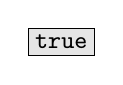
\begin{tikzpicture}
      \node [bddterminal] {$\true$};
    \end{tikzpicture}}
\newcommand{\bddfalse}[0]{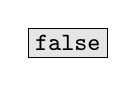
\begin{tikzpicture}
      \node [bddterminal] {$\false$};
    \end{tikzpicture}}


% Standardize command font styles and environments
\newcommand{\doccmd}[1]{\texttt{\textbackslash#1}}% command name -- adds backslash automatically
\newcommand{\docopt}[1]{\ensuremath{\langle}\textrm{\textit{#1}}\ensuremath{\rangle}}% optional command argument
\newcommand{\docarg}[1]{\textrm{\textit{#1}}}% (required) command argument
\newcommand{\docenv}[1]{\textsf{#1}}% environment name
\newcommand{\docpkg}[1]{\texttt{#1}}% package name
\newcommand{\doccls}[1]{\texttt{#1}}% document class name
\newcommand{\docclsopt}[1]{\texttt{#1}}% document class option name
\newenvironment{docspec}{\begin{quote}\noindent}{\end{quote}}% command specification environment



\begin{document}
\maketitle% this prints the handout title, author, and date

\begin{itemize}
  \item We have been filling in the PPL compilation picture which organizes 
  different kinds of probabilistic programming languages:

  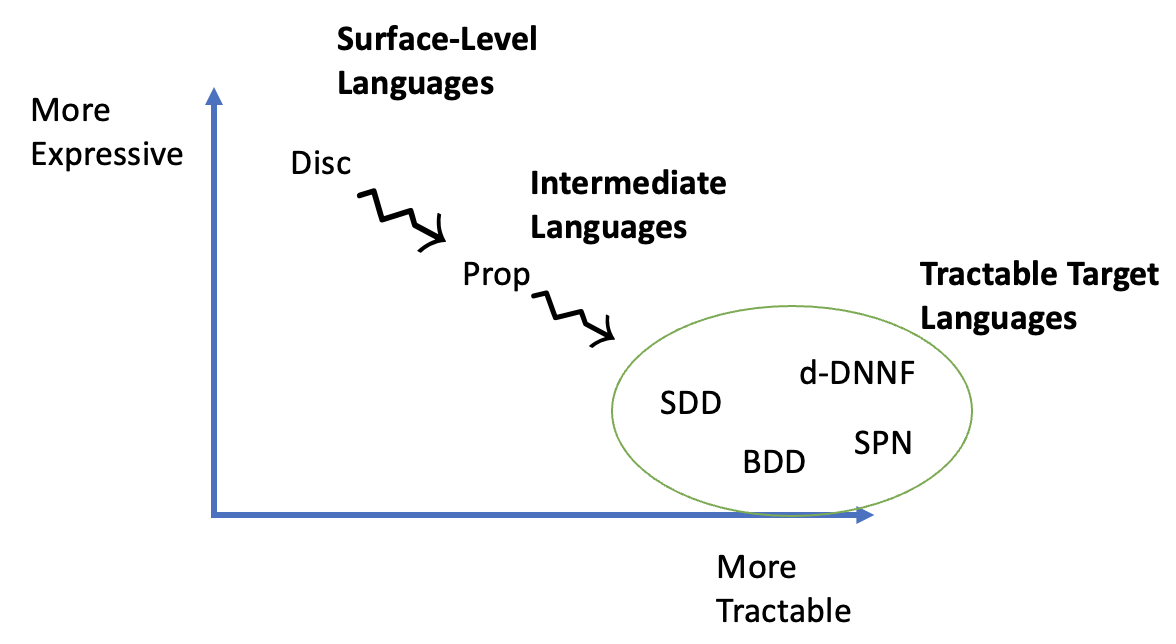
\includegraphics{motiv.png}

  \item We now understand every component. Recall:
  \begin{itemize}
    \item A language consists of syntax and semantics. We customarily give two 
    kinds of semantics: a denotational semantics that describes the mathematical 
    object associated with the program, and an operational semantics that tells
    us precisely how to compute that object. We typically prove something called
    ``adequacy'' that relates the denotational and operational semantics.
    \item A compilation $L_1 \compiles L_2$ is a procedure for translating programs 
    written in language $L_1$ into $L_2$ that preserves semantics.
    \item Language $L_1$ is more expressive than $L_2$ if we can efficiently 
    compile any program from $L_2$ into $L_1$ but not vice versa;
    \item We can compare tractability of languages based on their worst-case
    runtime complexity.
  \end{itemize}

  \item Some bibliographic notes: 
  \begin{itemize}
    \item The process of compiling a Boolean formula into a tractable target is
      often called \emph{knowledge compilation} in the
      literature~\citep{darwiche2002knowledge}. There are many tools for compiling 
      formulae. Some knowledge compilation tools:
      \begin{itemize}
        \item c2d compiles from CNF to d-DNNF: \url{http://reasoning.cs.ucla.edu/c2d/}
        \item minic2d compiles from CNF to SDD: \url{http://reasoning.cs.ucla.edu/minic2d/}
        \item rsdd compiles from Prop to SDD and BDD: \url{https://github.com/neuppl/rsdd}
        \item sharpSAT compiles from CNF to d-DNNF \citep{muise2012d}
      \end{itemize}
    \item Disc is based on Dice~\citep{holtzen2020scaling}. There are other PPLs
    that work by knowledge compilation, such as
    ProbLog~\citep{fierens2015inference,de2007problog},
    SPPL~\citep{saad2021sppl}. Historically, inference via compilation has been 
    very effectively used in inference for graphical models~\citep{chavira2008probabilistic,sang2005performing}
  \end{itemize}

  \item What are some research questions in here?
  \begin{itemize}
    \item Optimizing compilers for each stage.
    \item New tractable target languages.
    \item Compilation with performance guarantees.
    \item Tools for making building these compilers.
  \end{itemize}
\end{itemize}

\section{\disc{}: A simple discrete PPL}

\begin{itemize}
  \item Syntax:
\begin{lstlisting}[mathescape=true]
  e ::=
  | x $\leftarrow$ e; e
  | flip q                         // q is a rational value
  | if e then e else e
  | return e
  | true | false
  | e $\land$ e | e $\lor$ e | $\neg$ e |
  | ( e )
p ::= e
\end{lstlisting}

\item \disc{} looks very similar to a standard functional programming language,
but has two some interesting new keywords: \texttt{flip}, \texttt{observe}, and
\texttt{return}

\item $\texttt{flip}~\theta$ allocates a new random quantity that is $\true$
with probability $\theta$ and $\false$ with probability $1-\theta$

\item \texttt{return e} turns a non-probabilistic quantity into a probabilistic one, i.e. 
\texttt{return true} is a \emph{probabilistic quantity} that is $\true$ with probability 1 and 
$\false$ with probability 0

\item Example program and its interpretation: 

\begin{lstlisting}[mathescape=true]
x $\leftarrow$ flip 0.5; 
y $\leftarrow$ flip 0.5;
return x $\land$ y
\end{lstlisting}

This program outputs the probability distribution $[\true \mapsto 0.25, \false
\mapsto 0.75]$.

\item \textbf{Type system}: terms can either be pure Booleans of type $\bool$ 
or distributions on Booleans of type $\dist{\bool}$. So, we have the following 
type definition:
\begin{align}
  \tau ::= \bool \mid \dist{\bool}.
\end{align}

\item We define a typing judgment $\Gamma \vdash \te : \tau$ that associates each 
term with a type. The typing context $\Gamma$ is a map from identifiers to types.
\begin{mathpar}
  \inferrule{}{\Gamma \vdash \true{} : \bool} \and 
  \inferrule{}{\Gamma \vdash \false{} : \bool} \and
  \inferrule{}{\Gamma \vdash \texttt{flip}~\theta : \dist{\bool}} \and 
  \inferrule{\Gamma \vdash \te : \bool}{\Gamma \vdash \texttt{return}~\te : \dist{\bool}} \and
  % \inferrule{\Gamma \vdash \te_1 : \bool \and \Gamma \vdash \te_2 : \tau}
  %   {\Gamma \vdash \texttt{observe}~\te_1; \te_2 : \tau} \and
  \inferrule{\Gamma \vdash \te_1 : \dist{\bool} \and \Gamma \cup [x \mapsto \bool] \vdash \te_2 : \tau}
    {\Gamma \vdash x \leftarrow \te_1; \te_2 : \dist{\tau}} \and 
  \inferrule{\Gamma \vdash \te_1 : \bool \and \Gamma \vdash \te_2 : \tau \and \Gamma \vdash \te_3 : \tau}
    {\Gamma \vdash \texttt{if}~\te_1~\texttt{then}~\te_2~\texttt{else}~\te_3 : \tau} \and
  \inferrule{\Gamma \vdash \te_1 : \bool \and \Gamma \vdash \te_2 : \bool}
    {\Gamma \vdash \te_1 \land \te_2 : \bool}
\end{mathpar}

\item This is often called a \emph{monadic} type
system~\citep{moggi1991notions}; it waas introduced as a way of handling effects
in purely functional languages. We won't get too into monads yet. If 
you're curious, see \citet{ramsey2002stochastic}.

\end{itemize}



\subsection{Denotational semantics of \disc{}}

\begin{itemize}
\item We will define our denotation on \emph{closed terms}, i.e. terms with 
  no free variables in them. 
\item There are two kinds of terms: \emph{probabilistic} and \emph{pure} terms. 
Probabilistic terms have type $\dist{\bool}$, and pure terms have type $\bool$.
\item The denotational semantics of pure terms is standard: they map closed
  terms to Boolean values. Examples of closed terms:
  \begin{align*}
    \dbracket{\true} &= \true \\ 
    \dbracket{\false} &= \false \\ 
    \dbracket{\te_1 \land \te_2} &= \dbracket{\te_1} \land \dbracket{\te_2}
  \end{align*}
\item The denotational semantics of probabilistic terms maps closed terms 
to probability distributions, $\dbracket{\te} : \texttt{Bool} \rightarrow [0, 1]$,
and has the following inductive definition:

\begin{align*}
\dbracket{\texttt{flip}~\theta}(v) &= 
\begin{cases}
\theta& \quad \text{if }v = T\\
1-\theta& \quad \text{if }v = F\\
\end{cases}
 \\
 \dbracket{\texttt{return}~\te}(v) &= 
 \begin{cases}
 1\quad& \text{if }v = \dbracket{\te}\\
 0\quad&  \text{otherwise}\\
 \end{cases}
 \\
\dbracket{x \leftarrow \te_1; \te_2}(v) &= \sum_{v'} \dbracket{\te_1}(v') \times \dbracket{\te_2[v'/x]}(v)
\\
\dbracket{\texttt{if}~\true~\texttt{then}~\te_1~\texttt{else}~\te_2} &= \dbracket{\te_1} \\
\dbracket{\texttt{if}~\false~\texttt{then}~\te_1~\texttt{else}~\te_2} &= \dbracket{\te_2}
\end{align*}

\item Recall our notation for substitution $\te[v/x]$, which substitutes the 
  variable $x$ for value $v$. Here we define substitution to 
  be \emph{capture-avoiding}. This concept is best illustrated by example. 
  Considering the following program:
\begin{lstlisting}[mathescape=true]
x $\leftarrow$ true;
x $\leftarrow$ false;
return true
\end{lstlisting}
  What should this program return? Intuitively, it should return the 
  distribution $[\false \mapsto 1, \true \mapsto 0]$. 

\item A substitution $\te[v/x]$ is \emph{capture-avoiding} if it only
substitutes \emph{free occurrences} of $x$ with $v$ in $\te$. 
A variable is \defn{free} if it does not occur inside of a binding.
We can 
accomplish this with the following inductive description of substitution
(here we show only a subset of the rules):
\begin{mathpar}
  \inferrule{}{\true[x/v] = \true}
  \and
  \inferrule{}{\false[x/v = \false]}
  \and
  \inferrule{}{x[x/v] = v}
  \and 
  \inferrule{x \ne y}{y[x/v] = y}
  \and
  \inferrule{}{(x \leftarrow \te_1; \te_2)[v/x] = x \leftarrow \te_1[v/x]; \te_2}
  \and
  \inferrule{x \ne y}{(x \leftarrow \te_1; \te_2)[v/x] = y \leftarrow \te_1[v/x]; \te_2[v/x]}
\end{mathpar}

  % The interest case happens in the bind rule $x \leftarrow \te; \te$. Here, we
  % have to check and ensure that we are only substituting free occurrences.

  \item In your project, we have implemented capture-avoiding substitution for terms in Disc 
  for you.

\item A simple example of the let-rule:
\begin{align*}
  \dbracket{x \leftarrow \texttt{flip}~\theta; \texttt{return}~x}(\true) &= 
  \sum_{v \in \bool} \dbracket{\texttt{flip}~\theta}(v) \times \dbracket{\texttt{return}~v}(\true) 
  = \theta
\end{align*}


\end{itemize}

% \subsection{Inference via enumeration}
% \begin{itemize}
%   \item Define a relation $\te \Downarrow^e $
% \end{itemize}

\section{Compiling \disc{} to \prop{}}
\begin{itemize}
  \item \textbf{Goal}: give a semantics-preserving compilation
  $\rightsquigarrow$ that compiles \disc{} to \prop{}.
  \item We want to define this relation to satisfy the following
  \textbf{adequacy condition}, assuming the program $\te \compiles \prog$:
  \begin{align} 
    \dbracket{\te}(\true) = \dbracket{\prog}.
  \end{align} 
  % We will shorten this description to $\te \compiles
  % (\varphi, \varphi_A, w)$ and assume that the two formulae share a common
  % $w$. The adequacy condition then becomes:
  % \begin{align} 
  %   \dbracket{\te}_D(\true) = \frac{\dbracket{(\varphi, w)}}{\dbracket{(\varphi_A, w)}}.
  % \end{align} 
  \item Compilation relation:
  \begin{mathpar}
    \inferrule{}{\true \compiles (\true, \emptyset)} \and 
    \inferrule{}{\false \compiles (\false, \emptyset)} \and 
    \inferrule{}{x \compiles (x, [x \mapsto 1/2, \overline{x} \mapsto 1/2])} \and 
    \inferrule{\texttt{fresh}~f}
      {\texttt{flip}~\theta \compiles (f, [f \mapsto \theta, \overline{f} \mapsto 1-\theta])} \and
    \inferrule{\te_1 \compiles (\varphi, w) \and \te_2 \compiles (\varphi', w')}
      {x \leftarrow \te_1; \te_2 \compiles (\varphi'[\varphi/x], w_1 \cup w_2)} \and
    \inferrule{\te_1 \compiles (\varphi_1, w_1) \and \te_2 \compiles (\varphi_2, w_2)}
      {\te_1 \land \te_2 \compiles (\varphi_1 \land \varphi_2, w_1 \cup w_2)}\\
    \inferrule{\te_1 \compiles (\varphi_1, w_1) \and \te_2 \compiles (\varphi_2, w_2) \and 
    \te_3 \compiles (\varphi_3, w_3)
    }
    {\texttt{if e$_1$ then e$_2$ else e$_3$} \compiles 
    ((\varphi_1 \land \varphi_2) \lor (\neg \varphi_1 \land \varphi_3), w_1 \cup w_2 \cup w_3)}
  \end{mathpar}

  \item One thing to notice above: we have a new substitution rule
  $\varphi'[\varphi/x]$ that substitutes $x$ with an \emph{arbitrary
  propositional formula} $\varphi$ in $\varphi'$. For example:
  \begin{align*}
    (x \lor y)[z \land w/x] = (x \land y) \lor y.
  \end{align*}

  You can perform this operation directly on BDDs; it is called \emph{BDD
  composition}.

  \item Now we are almost ready to state the semantics-preservation property of
  this compilation. We need one extra piece: \emph{environment substitution}.
  \item Suppose $\Gamma \vdash \te$. A substitution $\gamma \in \dbracket{\Gamma}$ 
  gives an assignment to every free variable in $\te$. We use the notation 
  $\te[\gamma]$ to denote performing the substituting of all variables 
  in $\gamma$ in $\te$, i.e.:
  \begin{align*}
    \te[\{[v_1/x_1, v_2/x_2, \dots, v_n/x_n]\}] = \te[v_1/x_1][v_2/x_2]\dots[v_n/x_n].
  \end{align*}
  Additionally, note that we can apply this same substitution notation to 
  propositional formulae, i.e. $\varphi[\gamma]$ is also well-defined 
  according to the above description.
\end{itemize}

\begin{theorem}
Assume $\Gamma \vdash \te$ and $\te \compiles \prog$. Then, for any substitution
$\gamma \in \dbracket{\Gamma}$, is is the case that 
$\dbracket{\te[\gamma]}(\true) = \dbracket{\prog[\gamma]}$.
\end{theorem}
\begin{proof}
  The proof is on structural induction on terms in $\te$. 

  The base case for \texttt{flip} is simple but a good place to start. Assume $\texttt{flip}~\theta 
  \compiles (f, [f \mapsto \theta, \overline{f} \mapsto 1-\theta])$. Then,
  \begin{align*}
    \dbracket{\texttt{flip}~\theta}(\true) = \theta =  \dbracket{(f, [f \mapsto \theta, \overline{f} \mapsto 1-\theta])}.
  \end{align*}

  The critical case is the inductive step for binding. Inductive hypothesis:
  assume that $\te_1 \compiles (\varphi_1, w_1)$ and $\te_2 \compiles (\varphi_2, w_2)$, 
  and that for any well-typed substitution $\gamma$ it is the case that:
  \begin{itemize}
    \item $\dbracket{\te_1[\gamma]}(\true) = \dbracket{\varphi_1[\gamma]}$
    \item $\dbracket{\te_2[\gamma]}(\true) = \dbracket{\varphi_2[\gamma]}$
  \end{itemize}
  We need to show that $\dbracket{x \leftarrow \te_1; \te_2}(\true) =
  \dbracket{\varphi_2[\varphi_1/x], (w_1 \cup w_2)}$.

  \textbf{TODO}; if you want, you can take a peek at \citet{holtzen2020scaling}

\end{proof}

\begin{itemize}
  \item Question: Is this an efficient compilation? \emph{Yes}.
\end{itemize}

\section{Observation}
\begin{itemize}
  \item \texttt{observe} is a powerful keyword that lets us \emph{condition} the
program. For instance, suppose I want to model the following scenario: ``flip 
two coins and observe that at least one of them is heads. What is the probability 
that the first coin was heads?''

We can encode this scenario as a \disc{} program:

\begin{lstlisting}[mathescape=true]
x $\leftarrow$ flip 0.5; 
y $\leftarrow$ flip 0.5;
observe x $\lor$ y;
return x
\end{lstlisting}

This program outputs the probability distribution:
\begin{align*}
  [\true \mapsto (0.25 + 0.25) / 0.75, \false
\mapsto 0.25 / 0.75]
\end{align*} 

\item These semantics give an unnormalized distribution. The main semantic object of interest is 
the normalized distribution, which is given by the \defn{normalized semantics}:

$$
[\![e]\!]_D(T) = \frac{[\![e]\!](T)}{[\![e]\!](T) + [\![e]\!](F) },
$$


defined analogously for the false case.
  \item In order to handle observations, we will compile \disc{} programs into 
  \emph{two} \prop{} programs: one that computes the unnormalized probability of 
  returning $\true$, and one that computes the probability of evidence (i.e. normalizing constant)
  \item Inductive description has the shape $\te \compiles (\texttt{p}_1, \texttt{p}_2)$. 

  \item Compilation relation:
  \begin{mathpar}
    \inferrule{}{\true \compiles (\true, \true, \emptyset)} \and 
    \inferrule{}{\false \compiles (\false, \true, \emptyset)} \and 
    \inferrule{}{x \compiles (x, \true, \emptyset)} \and 
    \inferrule{\texttt{fresh}~x}
      {\texttt{flip}~\theta \compiles (x, \true, [x \mapsto \theta, \overline{x} \mapsto 1-\theta])} \and
    \inferrule{\te_1 \compiles (\varphi, \varphi_A, w) \and \te_2 \compiles (\varphi', \varphi_A', w')}
      {x \leftarrow \te_1; \te_2 \compiles (\varphi'[\varphi/x], \varphi_A'[\varphi/x] \land \varphi_A, w_1 \cup w_2)} \and
    \inferrule{\te_1 \compiles (\varphi, \varphi_A, w) \and \te_2 \compiles (\varphi', \varphi_A', w')}
      {\texttt{observe}~\te_1; \te_2 \compiles (\varphi', \varphi_A' \land \varphi_A, w_1 \cup w_2)}
  \end{mathpar}


\end{itemize}

$$
[\![\texttt{observe}~e_1; e_2]\!](v) = 
\sum_{\{v' \mid [\![{e_1}(v') = T\}]\!]} [\![{e_2}]\!](v)
$$

\begin{theorem}[Adequacy]
  For well-typed term $\te$,
  assume $\te \compiles (\varphi, \varphi_A, w)$. Then, 
  $\dbracket{\te}_D(\true) = {\dbracket{(\varphi, w)}} / {\dbracket{(\varphi_A, w)}}$.
\end{theorem}



\bibliographystyle{plainnat}
\bibliography{../bib}


\end{document}